\chapter{LHCb}
\label{chap:LHCb}

\section{LHC}
\label{sec:LHC}
The Large Hadron Collider (LHC) is the world's largest and most powerful particle accelerator. Located at CERN (\textit{European Organization for Nuclear Research}), it consists of a 27 km ring of superconducting magnets with a number of accelerating structures, that boost the energy of the particles along the way. 

Two proton beams travelling in opposite directions collide at different points of the ring. These are extracted from ion sources, and accelerated in a chain of preaccelerators, being the lat stage of such chain the Super Proton Synchrotron (SPS) (see \figref{fig:LHC}). 
They are accelearted to produce collisions at energy in the center of mass ($\sqrt{s}$) of the order of the TeV, in order to test the Standard Model and look for New Physics. One of its main achievements has been the discovery of the Higgs boson, introduced in~\cite{Chatrchyan:2012xdj},~\cite{Aad:2012tfa}, the last piece of the Standard Model puzzle. Protons are sent on bunches containing up to $1.5\times 10^{11}$ particles, and corssing with a rate of 40 MHz. Special runs with heavy ions (e.g. lead) are also made periodically. 
\begin{figure} [htb!]
\begin{center}
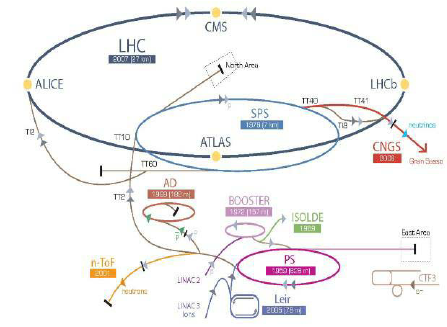
\includegraphics[scale=0.5]{figs/lhc.png}
\caption{The LHC injection complex. \label{fig:LHC}}
\end{center}
\end{figure}

%% Runs 
Since it first started operating in 2008, it has recorded data with different center of mass energies, corresponding to 2 data-taking periods: Run 1 (2009-2013,  $\sqrt{s}$ = 7, 8 TeV), and Run 2 (2013-present, $\sqrt{s}$ = 13, 14 TeV). An upgrade of the detectors was made in between the runs. 
%% Experiments

There are four interaction points within the LHC ring, corresponding to the four main experiments. In these points, the beams cross over to the other beam pipe and collide under a small angle. These four experiments are: 

\begin{itemize}
\item \textbf{ATLAS} (\textit{A Toroidal LHC ApparatuS})~\cite{Armstrong:1994it}: a general-purpose 4$\pi$ detector, focused mainly in the search of New Physics via direct searches and responsible of the Higgs boson discovery.
\item \textbf{CMS} (\textit{Compact Muon Solenoid})~\cite{CMS:1994hea}: also a general-purpose detector, with a physics program similar to ATLAS and a more compact layout. 
\item \textbf{ALICE} (\textit{A Large Ion Collider Experiment})~\cite{Alice}: the smallest of the four detector, it focuses in heavy-ion studies. 
\item \textbf{LHCb} (\textit{Large Hadron Collider beauty})~\cite{Amato:1998xt}: a single-arm forward spectrometer, initially designed for the study of particles containing \bquark or \cquark quarks, now converted into a general-purpose detector. It is described in more detail in the following section. 
\end{itemize}


\section{LHCb}
\label{sec:LHCb}


The \lhcb detector~\cite{Alves:2008zz,Aaij:2014jba} is a single-arm forward
spectrometer covering the \mbox{pseudorapidity} range $2<\eta <5$,
designed for the study of particles containing \bquark or \cquark
quarks. The detector includes a high-precision tracking system
consisting of a silicon-strip vertex detector surrounding the $pp$
interaction region~\cite{LHCb-DP-2014-001}\verb!*!, a large-area silicon-strip detector located
upstream of a dipole magnet with a bending power of about
$4{\mathrm{\,Tm}}$, and three stations of silicon-strip detectors and straw
drift tubes~\cite{LHCb-DP-2013-003}\verb!*! placed downstream of the magnet.
The tracking system provides a measurement of the momentum, \ptot, of charged particles with
a relative uncertainty that varies from 0.5\% at low momentum to 1.0\% at 200\gevc.
The minimum distance of a track to a primary vertex (PV), the impact parameter (IP),
is measured with a resolution of $(15+29/\pt)\mum$,
where \pt is the component of the momentum transverse to the beam, in\,\gevc.
Different types of charged hadrons are distinguished using information
from two ring-imaging Cherenkov detectors~\cite{LHCb-DP-2012-003}\verb!*!.
Photons, electrons and hadrons are identified by a calorimeter system consisting of
scintillating-pad and preshower detectors, an electromagnetic
calorimeter and a hadronic calorimeter. Muons are identified by a
system composed of alternating layers of iron and multiwire
proportional chambers~\cite{LHCb-DP-2012-002}\verb!*!.
The online event selection is performed by a trigger~\cite{LHCb-DP-2012-004}\verb!*!,
which consists of a hardware stage, based on information from the calorimeter and muon
systems, followed by a software stage, which applies a full event
reconstruction.

%%% LHC 
%%% LHCb : 
%% more details 
%% subdetector

\begin{figure} [htb!]
\begin{center}
%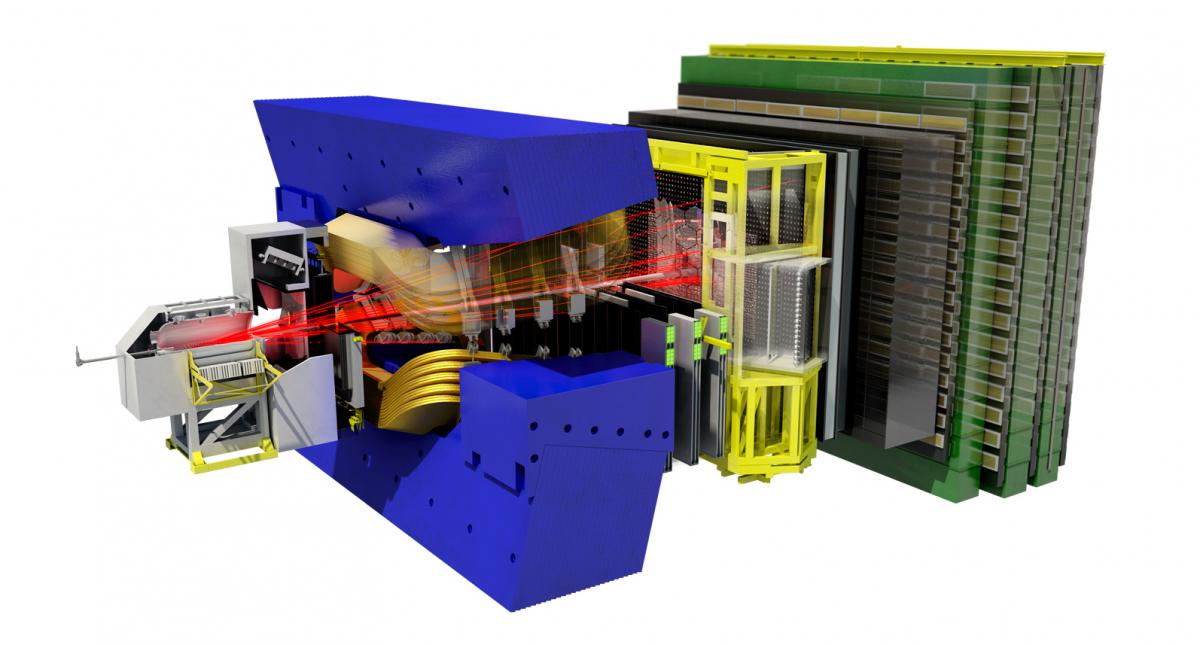
\includegraphics[scale=0.2]{figs/lhcb.jpg}
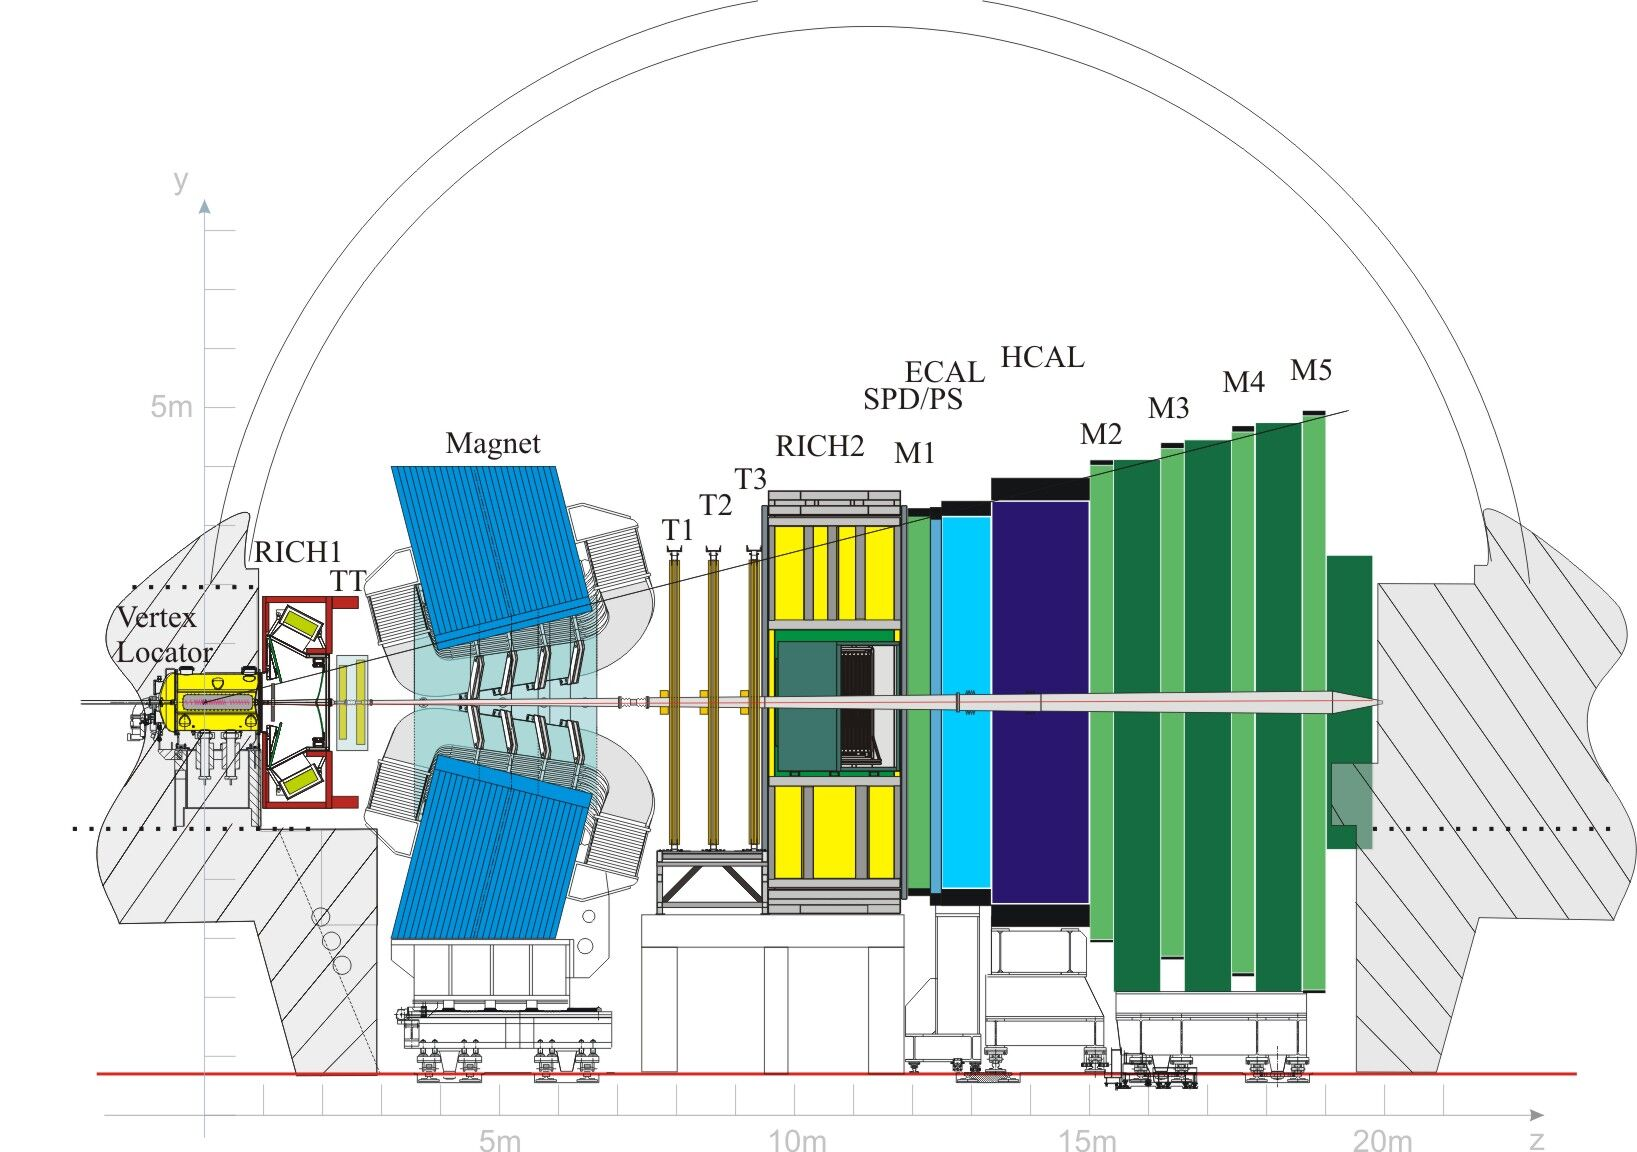
\includegraphics[scale=0.2]{figs/lhcb-slide.jpg}
\caption{LHCb detector \label{fig:LHCb}}
\end{center}
\end{figure}

\subsection{Beam pipe, vacuum chamber and BCM} % martes
The design of the beampipe (\ref{fig:beampipe}) is especially delicate, given the pseudorapidity region at which LHCb operates, where there is a high particle density. It is of 19m long and includes the forward window of the VELO and four main conical sectors. The three closer to the interaction point are made of beryllium, as it is highly transparent to particles resulting from collisions. The one left is made of stainless steel because of its good mechanical and vacuum properties. The beampipe support system consists of one fixed and one movable support, in order to reduce the background as much as possible. Two sector valves located at the cavern entrances isolate the experiment beam vaccum from the LHC.

The Beam Conditions Monitor (BCM) takes care of possible problems with the LHC beam conditions, requesting a beam dump if necessary. It monitors the particle flux at two locations close to the vacuum chamber (so as to protect the sensitive LHCb tracking devices). It is connected to the LHCb experiment control system and to the beam interlock controller of the LHC. The two stations consist of eight diamond sensors, with the same dimensions as those of ATLAS and CMS.
 
\begin{figure} [htb!]
\begin{center}
%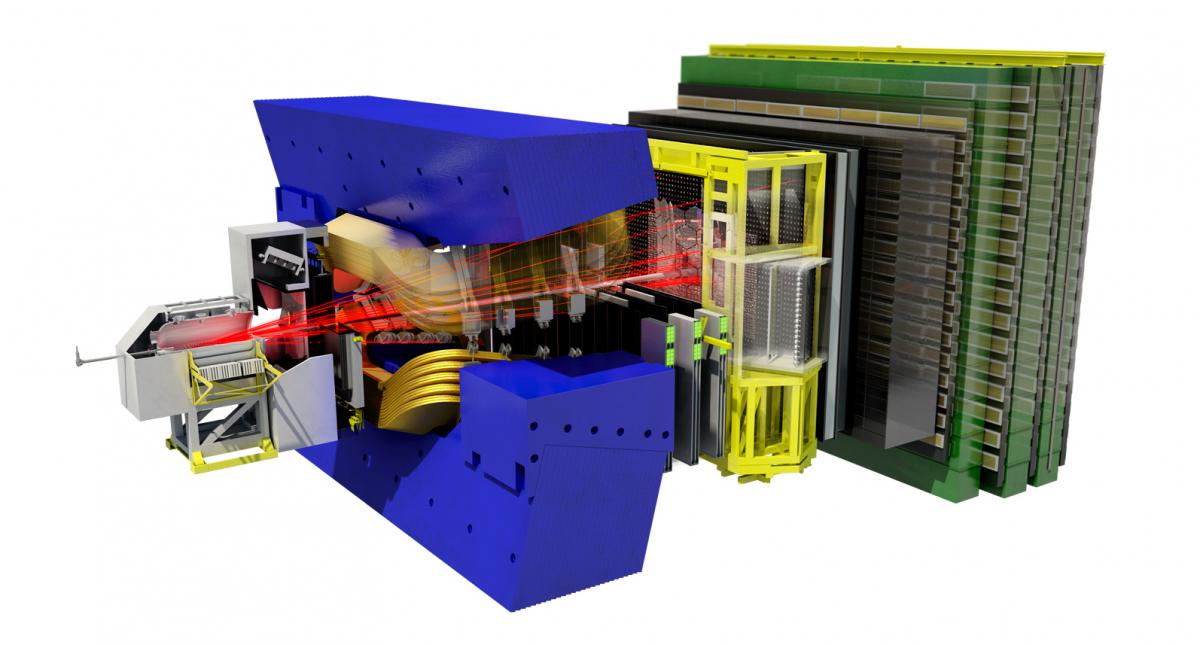
\includegraphics[scale=0.2]{figs/lhcb.jpg}
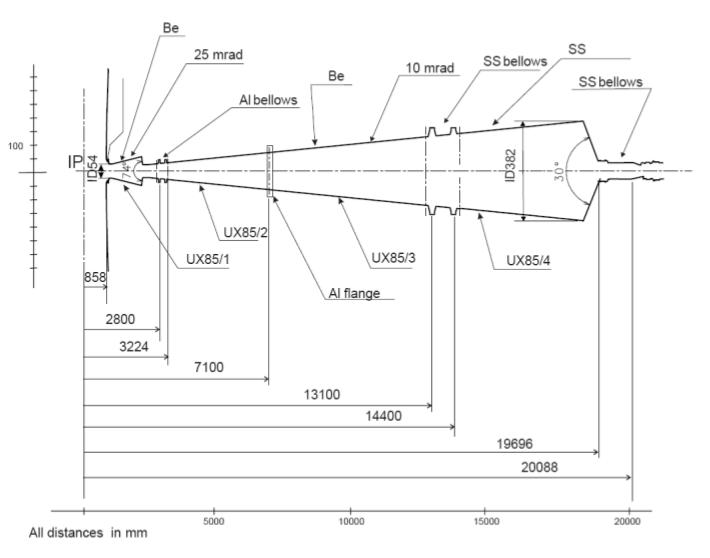
\includegraphics[scale=0.6]{figs/beampipe.png}
\caption{LHCb beam pipe \label{fig:beampipe}}
\end{center}
\end{figure}


\subsection{Magnet} % martes
LHCb contains a dipole magnet that bends charged particles in order to measure their momenta. The measurement covers the forward acceptance of $\pm 250 \rm mrad$ verticaly and of $\pm 300 \rm mrad$ horizontally. Two identical conical saddle-shaped coils surround an iron yoke, producing a magnetic field of 4 Tm for tracks of 10 m length (notice that difference parts of the detector need for different values of the magnetic field). These coils are made of pure Al-99.7. 

The magnet is operated using a Magnet Control System, a well as a Magnet Safety System, that takes care of the security of the magnet performance. 

The precision with which the magnetic field of the magnet is measured needs to be of the order of $10^{-4}$ so as to properly measure the momentum resolution of the charged particles. In order to ensure this, field mapping campaigns in the tracking volume were made and obtained a value of about $4\times 10^{-4}$ (\ref{fig:lhcbmagnet}). In order to reduce the systematic effects of the detector, especially for $CP$ studies, the polarity of the magnetic field needs to be changed periodically. 

\begin{figure} [htb!]
\begin{center}
%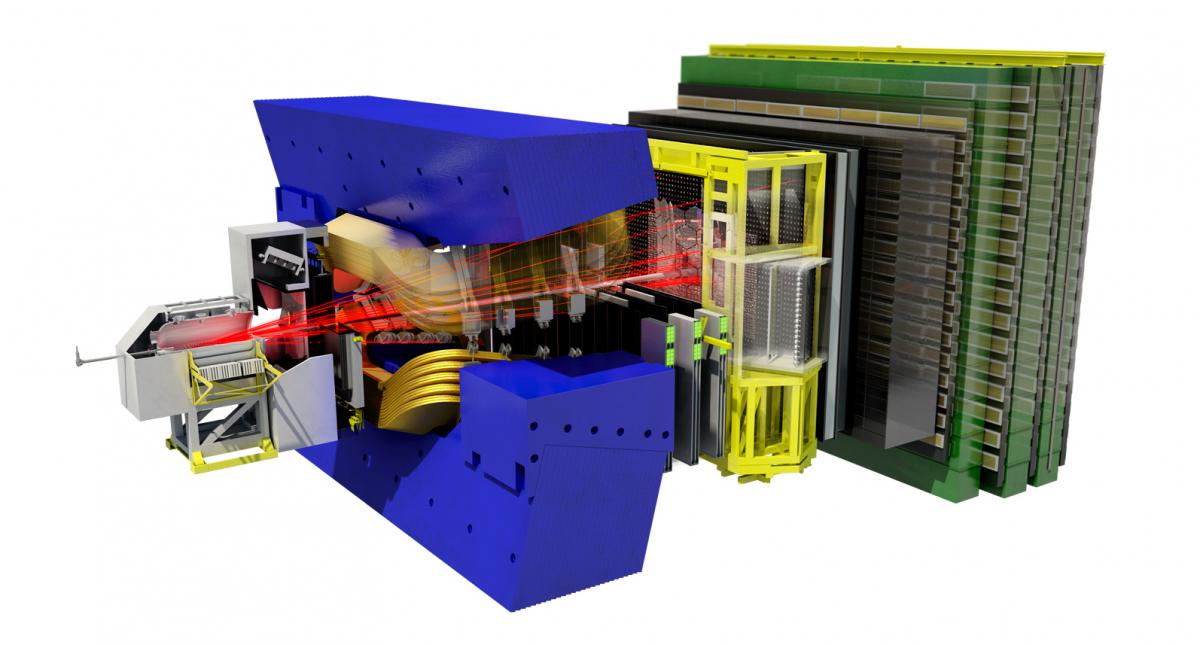
\includegraphics[scale=0.2]{figs/lhcb.jpg}
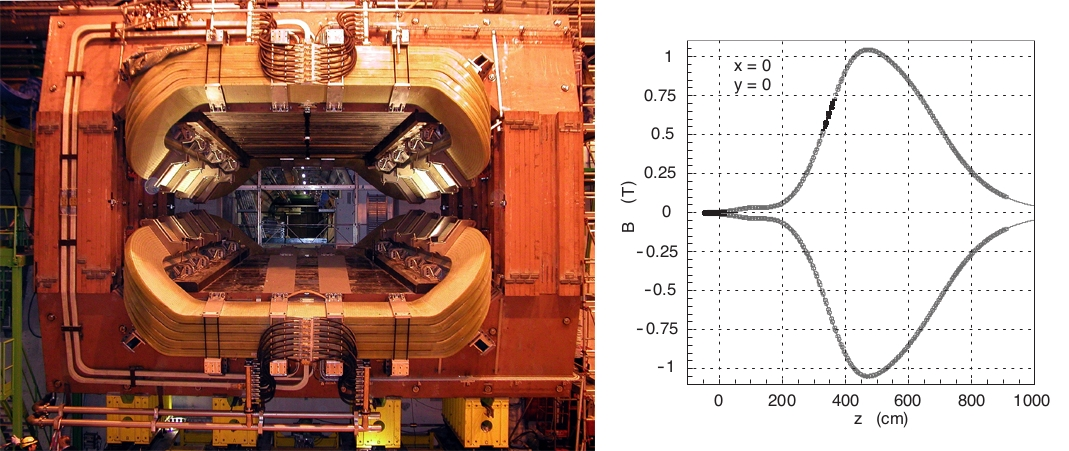
\includegraphics[scale=0.35]{figs/magnet.jpg}
\caption{LHCb magnet (left) and magnetic field along the z axis (right)\label{fig:lhcbmagnet}}
\end{center}
\end{figure}

\subsection{Tracking} %% martes, miercoles, jueves 
\label{sec:Tracking}
The tracking system of LHCb consists of two parts: the vertex locator (VELO) and four tracking stations: the \textit{Tracker Turicensis} (TT) upstream of the magnet, and T1-T3 downstream of the magnet. The latter are composed by an Inner Tracker (IT) and an Outer Tracker (OT). Both IT and TT belong to a common project, the \textit{Silicon Tracker} (ST). 

\subsubsection{VELO} 
The ability to reconstruct vertices with a high precision is a key feature of the LHCb detector. It is vastly used to accurately measure the decay lifetimes, the impact parameter and the flavour of the particles that are produced. Besides, detached vertices are of crucial importance for the High Level Trigger (\ref{sec:Trigger}). 

Such reconstruction is done in the VErtex LOcator (VELO), that provides measurements of the track coordinates close to the interaction region. It consists of 20 semicirular silicon modules located along the beam direction, each one providing measurement of cylindrical coordinates $(r,\phi)$ using microstrips, together with two planes perpendicular to the beam line, the \textit{pile-up veto system}, as it can be seen in \ref{fig:velo}, that are then used to get rid of high multiplicity events. The minimum pitch at the innermost radius
is $38  \rm \mu m$, increasing linearly to $101.6  \rm \mu m$ at the oter radius of 41.9mm . 
These sensors must be retractable, as the distance from them to the beam is smaller than the one required from LHC during the injection phase.  Vacuum inside the VELO is separated from the machine vacuum by corrugated aluminum foils, \textit{RF-foils}. 

The VELO was designed in order to fulfill the signal to noise ratio, efficiency, resolution and geometrical requirements. Polar coordinates are used in order to ensure fast reconstruction of tracks and vertices in the LHCb trigger~\cite{Alves:2008zz}.

\begin{figure} [htb!]
\begin{center}
%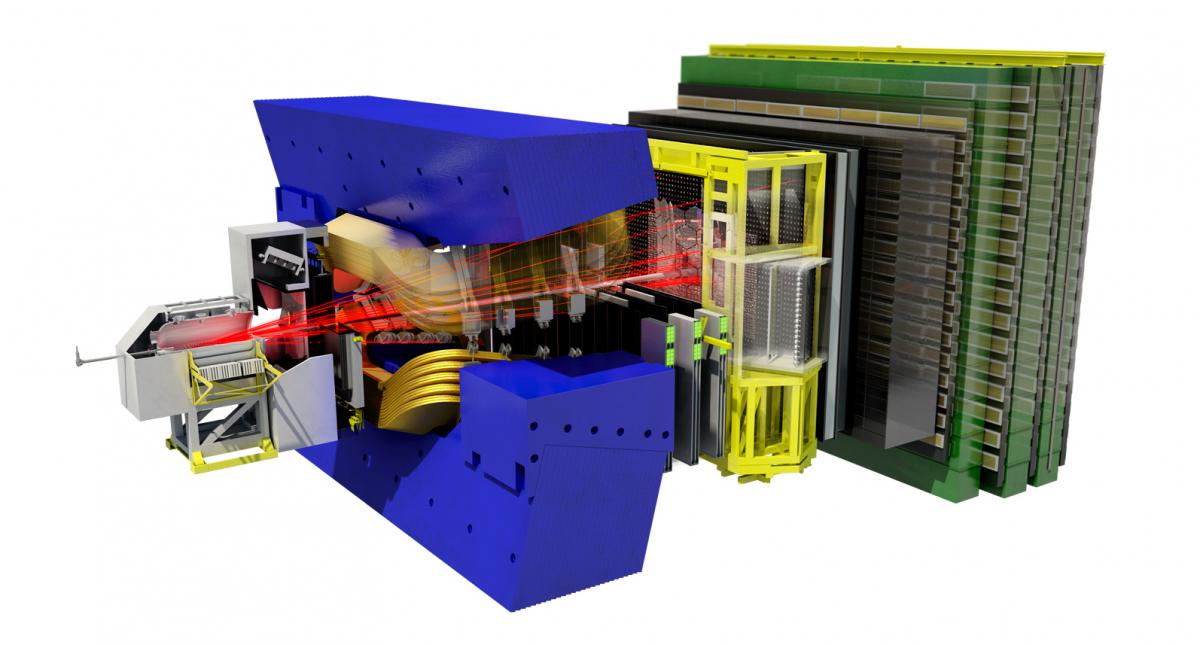
\includegraphics[scale=0.2]{figs/lhcb.jpg}
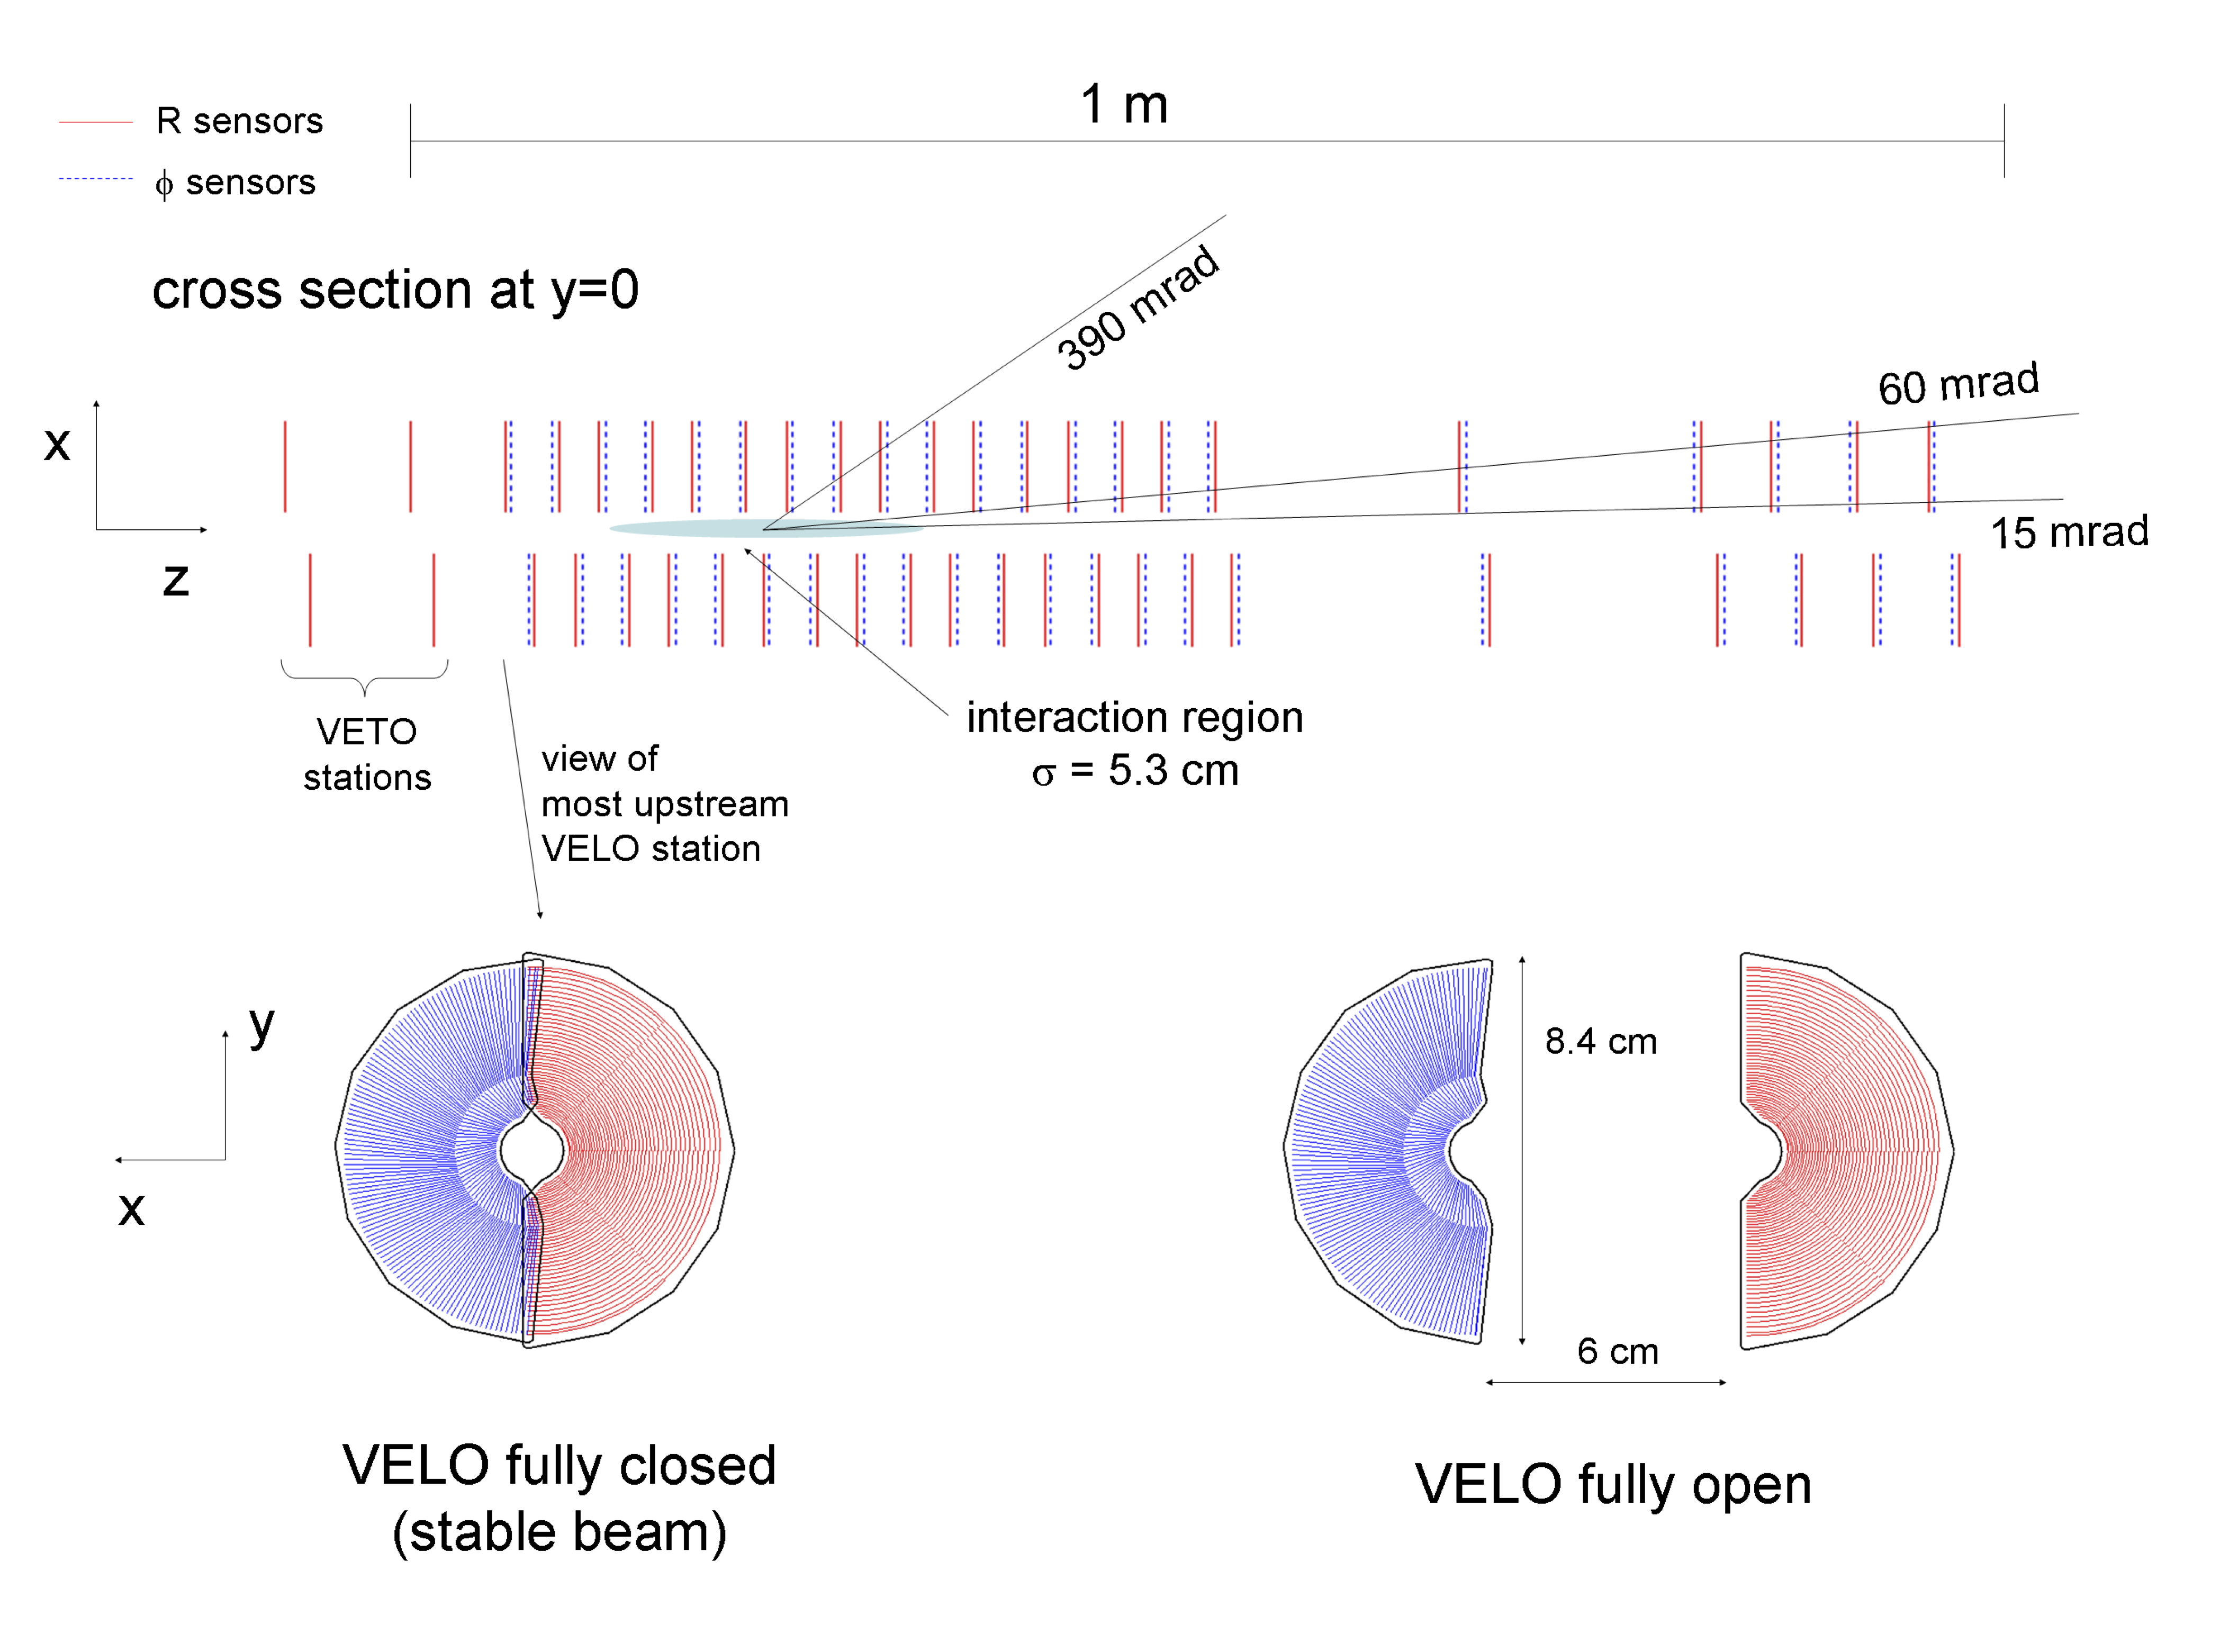
\includegraphics[scale=0.18]{figs/velo.png}
\caption{Cross section in the ($x$,$z$) plane of the VELO silicon sensors, at $y=0$, with the detector in the fully closed position. The front face of the first modules is also illustrated in both the closed and open positions~\cite{Alves:2008zz}.\label{fig:velo}}
\end{center}
\end{figure}

\subsubsection{ST} 
As said before, the Silicon Tracker (ST) refers to two different detectors: the Tracker Turicensis (formerly known as \textit{Trigger Tracker} (TT) and the Inner Tracker (IT) (see \ref{fig:lhcb_st}). Both use silicon microstrip sensors with a strip pitch of about 200 $\mu$m. 
The TT is a 150x130 cm high planar tracking station (covering the full LHCb acceptance), located upstream of the LHCb dipole magnet. The IT covers a 120x40 cm high cross shaped region in the centre of the three tracking stations downstream of the magnet. 

The TT and each of the three IT stations have four detection, organized in an (\textit{x-u-v-x}) configuration, with vertical strips in the first and the last layer. Strips in the second and third layer are rotated by a stereo angle of $-5^{\circ}$ and $5^{\circ}$ respectively (so as to get 3D reconstruction). The pitch is about $200\mu m$ which gives a single hit resolution of 50$\mu m$. Momentum resolution is then dominated by multiple scattering. The active area is of about $8.4m^2$ for the TT and of $4.0m^2$ for the IT. A temperature below $5^{\circ}\rm C$ is maintained in both cases.  

\begin{figure} [htb!]
\begin{center}
%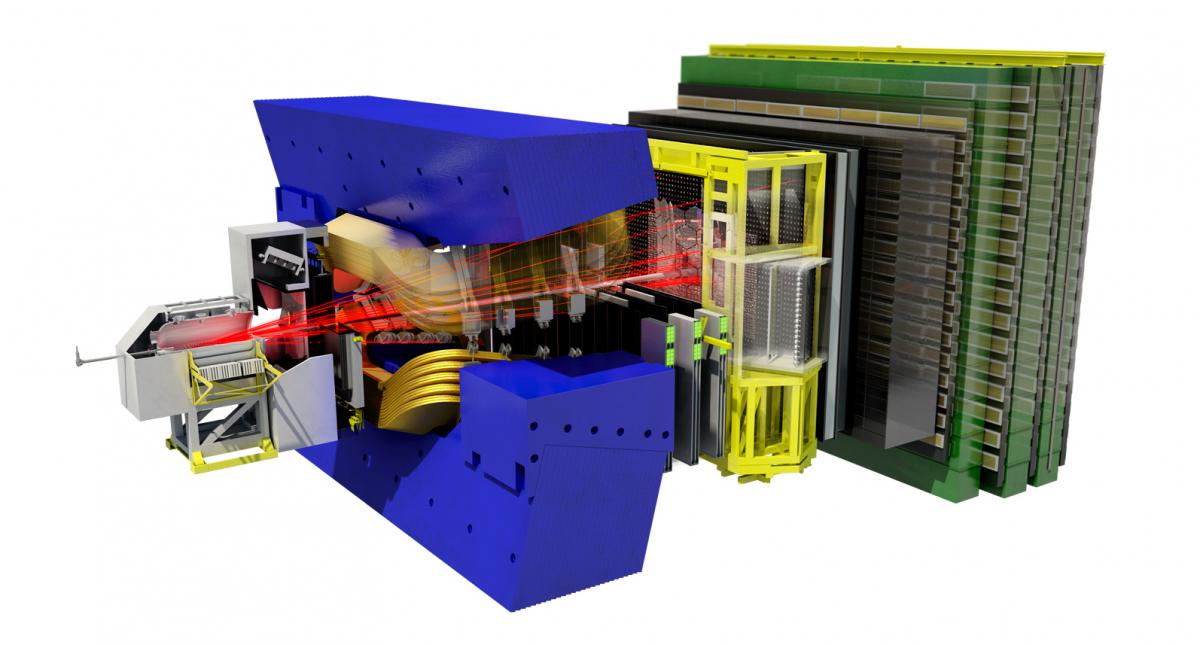
\includegraphics[scale=0.2]{figs/lhcb.jpg}
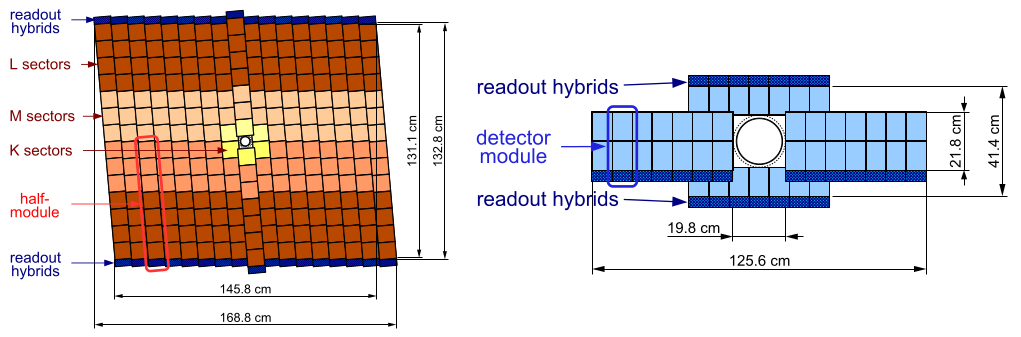
\includegraphics[scale=0.6]{figs/lhcb_st.png}
\caption{Layout of the third TT detection layer (left) and layout of an x detection layer in the second IT station (right)~\cite{Alves:2008zz}.\label{fig:lhcb_st}}
\end{center}
\end{figure}

\subsubsection{OT} % miercoles
The OT detector is designed for the tracking of charged particles, and the measurement of their momentum. Excellent momentum resolution and high tracking efficiency are needed for LHCb analyses. It consists \red{in} a drift-time detector, composed of an array of gas-tight straw-tube modules. For the gas, a mixture of Argon (70\%) and $CO_2$ (30\%) is used. This ensures a fast drift time, as well as a sufficient drift-coordinate resolution. 

The modules are arranged in three stations, each one consisting of four layers. The stations are further splitted in two halves, with two independently retractable units of two half layers (C-frames). Such arrrangement can be seen in \ref{fig:lhcb_ot}. 

\begin{figure} [htb!]
\begin{center}
%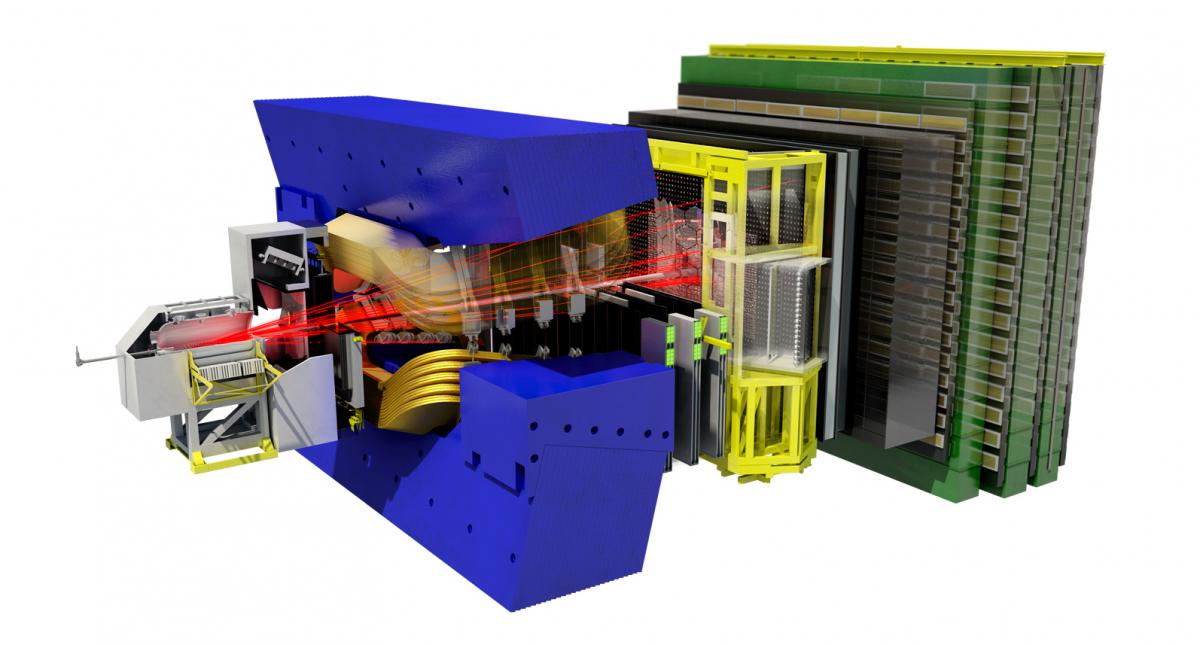
\includegraphics[scale=0.2]{figs/lhcb.jpg}
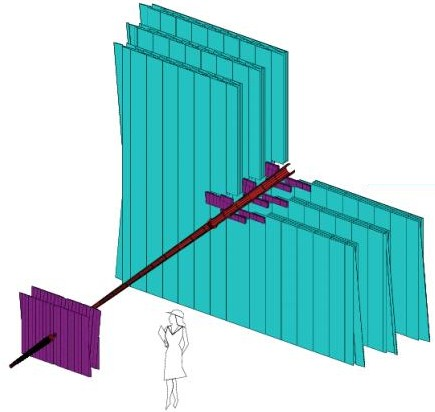
\includegraphics[scale=0.4]{figs/OT.jpg}
\caption{Arrangement of OT straw-tube modules in layer and stations~\cite{Alves:2008zz}.\label{fig:lhcb_ot}}
\end{center}
\end{figure}

\subsection{PID} % miercoles, jueves, viernes 
\label{sec:PID}
Particle identification (PID) at LHCb is crucial in order to properly distinguish the different types of particles that are detected. Particularly, it is important to further reduce backgrounds from different decays, as well as at the trigger level (\ref{sec:Trigger}). Three different subdetectors, described below, are used for PID.

\subsubsection{RICH}
There are two \textit{Ring Imaging Cherenkov detectors} at LHCb, designed to cover the full momentum range. RICH1 (\ref{fig:lhcb_rich} left) covers the low momentum charged particle range ($\sim 1-60 \rm GeV$), while RICH2 (\ref{fig:lhcb_rich} right) covers the high momentum charged particle range ($\sim 15\rm GeV$ up to and beyond $\sim 100\rm GeV$). In order to do this, RICH1 (located upstream, between the VELO and the Trigger Tracker) uses aerogel and $\rm C_4F_{10}$ radiators, while the downstream detector, RICH2, uses a $\rm CF_4$ radiator. 

While RICH1 covers the ful LHCb acceptance, from $\pm 25 \rm rad$ to $\pm 300 \rm rad$ horizontal and $\pm 250 \rm rad$ vertical, RICH2 has a more limited angular acceptance (where the high momentum particles are produced), of $\sim \pm 15 \rm rad$ to $\pm 120 \rm rad$ horizontal and $\pm 100 \rm rad$.

\begin{figure} [htb!]
\begin{center}
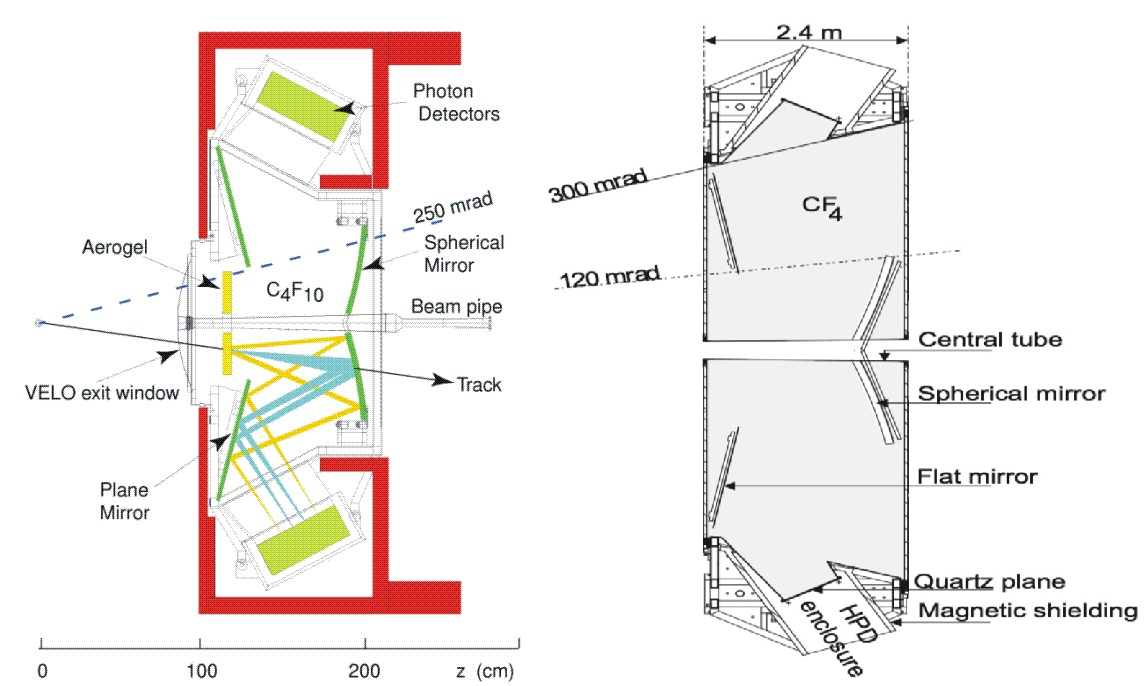
\includegraphics[scale=1.5]{figs/RICH.png}
\caption{Schematic view of  RICH1 (left) and RICH2 (right) detectors~\cite{Alves:2008zz}.\label{fig:lhcb_rich}}
\end{center}
\end{figure}

Both detector use spherical and flat mirrors to focus the Cherenkov light. The optical layout is vertical for RICH1 and horizontal for RICH2. Cherenkov photons in the wavelength range 200-600 nm are detected by Hybrid Photon Detectors (HPDs), which are outside the LHCb acceptnce. These are surrounded by external iron shields that shield tem from the marginal field of the LHCb dipole. 
%%% The spherical mirrors are located within the LHCB acceptance and are traversed by charged particles and photons 

\subsubsection{Calorimeters} % miercoles
The transverse energy of hadrons, electrons and photons is measured and selected in the calorimeter for the L0 trigger (\ref{sec:Trigger}). The energy and position is also measured for these particles, which are identified in this subdetector, while avoiding the pass of those particles to the muon system. The proper identification of hadrons, electrons and photons is also of great importance for correctly identifying the flavour of the original meson in the decay (\textit{flavour tagging}). This is done taking into account that these particles deposit the energy in the different parts of the calorimeter in a different manner. 
 
It consists of two separate parts: an electromagnetic calorimeter (ECAL) followed by a hadron calorimeter (HCAL), to identify electromagnetic and hadronic showers, respectively. A preshower detector (PS) is located before the ECAL, in order to eliminate a large background of charged pions that could be misidentified as elecrons. In front of the PS, a scintillator pad detector (SPD), used to select charged particles, is located. For all these parts a variable lateral segmentation is adopted, given that the hit density varies by two orders of magnitude over the calorimeter surface ~\cite{Alves:2008zz}. Because of the dimensions of the hadronic showers, the HCAL is segmented into two zones with larger cell sizes. 

In all cases, the same principle of scintillation light transmitted to a Photo-Multiplier (PMT) (that turn this light into an electric ignal) by wavelength-shifting (WLS) fibres is adopted. To have a constant transverse energy cale the gain in the ECAL and HCAL phototubes is set in proportion to their distance to the beampipe.  

\begin{figure} [htb!]
\begin{center}
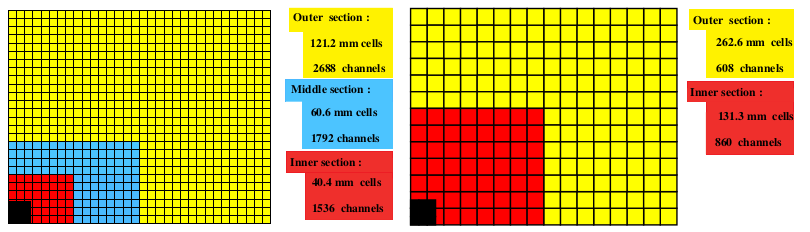
\includegraphics[scale=0.7]{figs/CALO.png}
\caption{Lateral segmentation of the SPD/PS and ECAL (left) and the HCAL (right). One quarter of the detector front face is shown~\cite{Alves:2008zz}.\label{fig:lhcb_calo}}
\end{center}
\end{figure}


%%\red{dimensions?}

\subsubsection{Muon System} 
The muon system provides fast information for the high-$p_T$ muon trigger at the earliest level (L0) and muon identification for the high-level trigger (HLT) and offline analysis~\cite{Alves:2008zz}. Given that muons are present in final states of the most relevant channels for LHCb, this is of crucial importance.

It is composed of five rectangular stations (M1-M5), located along the beam axis, with a total of 1380 chambers and 435$\rm m^2$ of coverage. The inner and outer angular acceeptances are 20(16) mrad and 306(258) mrad in the bending (non-bending) plane respectively~\cite{Alves:2008zz}. All the stations are divided into 4 regions, R1-R4, with increasing distance from the beam axis. Their dimensions (scaling a factor two  from one region to the next) and their geometry provide the same flux and channel ocupancy for all of them. Muti-wire proportional chambers (MWPC) are used for all regions except the inner region of station M1, where triple-GEM detectors (consisting of three gas electron multipliers) are used. 

Stations M2 to M5 are placed downstream the calorimeters, interleaved with three iron filters. They have a threshold of $\sim 6 \rm GeV/c$ for a muon to cross the five stations. Stations M1-M3 are used to define the track direction and to calculate the $p_T$ of the candidate muon, due to their high spatial resolution along the bending plane. Stations M4 and M5 are focused on identifying penetrating particles. Station M1 is located in front of the calorimeters. Its function is to improve the $p_T$ measurement in the trigger. The geometry of all the stations is such that all their transverse dimensions scale with the distance from the interaction point. %% A fourth station is situated after M5 to remove machine related background 


%%% The muon stations are equipped with Multi Wire Proportional Chambers [98] (MWPCs) operating
%% with an Ar:CO 2 :CF 4 (40%:55%:5 % in volume) gas mixture. The only exception to the MWPCs is the
%% innermost region R1 of the station M1, in which the high rate of particles requires the use of a triple-
%% GEM detector, which consists of three gas electron multiplier (GEM), using Ar:CO 2 :CF 4 (45%:15%:40%
%%% in volume) as a gas mixture.

\begin{figure} [htb!]
\begin{center}
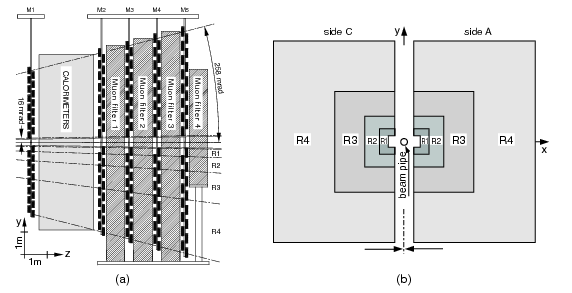
\includegraphics[scale=1.0]{figs/MUON.png}
\caption{(a) Side view of the LHCb Muon Detector. (b) Station layout with the four regions R1-R4~\cite{Alves:2012ey}.\label{fig:lhcb_muon}}
\end{center}
\end{figure}

\subsection{Trigger} 
\label{sec:Trigger}
The LHCb trigger is one of the most important part of its infrastructure, as it allows for a reduction of the crossing frequency with interactions visible by the spectrometer from 10MHz to about 2 - 5 kHz, at which rate the events are written to storage for further offline analysis~\cite{Alves:2008zz}. It is composed by two levels: Level-0 (L0) and the High Level Trigger (HLT). Both parts are optimised to obtain the highest efficiency for the events selected in the offline analysis, while avoiding storage of as much background events as possible. 

\subsubsection{L0}
The purpose of this first stage of the trigger is to reduce the LHC beam crossing rate of 40 MHz to 1MHz, with which the entire detector can be read out ~\cite{Alves:2008zz}. This is done reconstructing the highest $E_T$ hadron, electron and photon clusters in the calorimeters, together with the the two highest $p_T$ muons in the muon chambers, as B meson decay products are expected to have large $p_T$ and $E_T$. A pile-up system in the VELO estimates the number of primary pp interactions in each bunch crossing. The calorimeters calculate the total observed energy and an estimate for the number of tracks, based on the number of hits in the SPD. With this, unwanted events are discarded. 

It is composed by three parts, all connected to a different part of the LHCb, and all connected to the L0 DU (see \ref{fig:lhcb_L0}):

\begin{enumerate}
\item The pile-up system: its purpose is dinstinguishing crossings with single and multiple visible interactions. For this, it uses four silicon sensors as the ones used in the VELO, that measure the radial position of the tracks.  It consists of two silicon planes, situated upstream of the VELO and perpendicular to the beam-line, where the radii of track hits are measured.  From this, the position of the track origin on the beam axis (the \textit{vertex}) can be reconstructed.  %%%% two overlapping velo R-sensors which have strips at constant radii, and each strip covers 45 degrees
\item The L0 calorimeter trigger: its goal is to look for high $E_T$ electrons, photons, neutral pions or hadrons. This is done forming clusters by adding the transverse energy of 2x2 cells and selecting the cluster with the highest $E_T$. This zone is large enough to contin most of the energy, while avoiding overlapping among different particles. Afterwards, such cluster is identified as one of the particle types using information from the SPD, PS, ECAL and HCAL subdetectors. 
\item The L0 muon trigger: in the muon chambers muons are reconstructed with a resolution in $p_T$ of $\sim 20\%$. The L0 muon trigger selects the two muons with the highest $p_T$ for each quadrant of the muon detector. The track finding is performed on the logical pads, searching for hits defining a straight line through the fivve muon stations and pointing towards the interaction point~\cite{Alves:2008zz}, also enabling the determination of the $p_T$ of the track.  %%% Seeds of the track finding algorithm are hits in M3. For each logical pd hit in M3, an extrapolated position is set in M2, M3 and M5, long a straight line passing thorugh the hit and the interaction point. 
\end{enumerate}
Multiplicities are measured by the SPD cells.
%%\red{charged track multiplicity}

A L0 Decision Unit (DU) collects all the information and derives the final L0 trigger decision for each bunch crossing to the Readout Supervisor , allowing for overlapping of several trigger conditions, as well as for prescaling. The Readout Supervisor is in chrage of the ultimate decision about whether to accept an event or not. 

The L0 uses custom made electronics, fully synchronous with the 40 MHz bunch crossing signal of the LHC. All L0 electronics uses fully custom-designed boards that use parallelism and pipelining in order to speed up the process. The time passed between a pp interaction and the arrival of the L0 trigger decision is of 4 $\mu$s, that leaves 2$\mu$s for data processing in the L0.

\begin{figure} [htb!]
\begin{center}
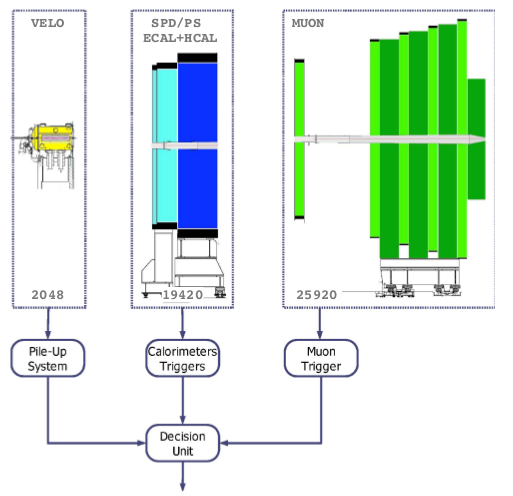
\includegraphics[scale=0.7]{figs/L0.png}
\caption{Overview of the L0~\cite{Alves:2008zz}.\label{fig:lhcb_L0}}
\end{center}
\end{figure}



\subsubsection{HLT} 
%% processor farm
The High Level Trigger (HLT) reduces the event rate from 1MHz down to 2 - 5 kHz, making use of the full event data. The HLT selected events are then saved on permanent storage. The algorithms that it uses refine candidates found by the L0 and divide them into independent \textit{alleys}, selected from the L0 decision, requiring the candidate tracks to be reconstructed in the VELO and/or the T-tations. With this, the rate is reduced to about 30kHz, where it becomes interesting to take into account both inclusive and exclusive criteria. It is further subdivided into HLT1 and HLT2, each with different purposes. The overall flow of all the trigger steps can be seen in \ref{fig:lhcb_HLT}. 

It consists of a C++ application that runs on over \red{2000} computing nodes, the Event Filter Farm (EFF). Even though it can access all data in one event, the purpose is to discard uninteresting event using part of the full event data. The cuts applied at this stage are generally very loose compared to the offline analysis, so as to be able to study the sensitivity of the selections and to profit from refinements due to improved calibration constants. In order to compute systematic uncertainties and trigger efficiencies, both levels can be fully emulated on stored data. 

\begin{figure} [htb!]
\begin{center}
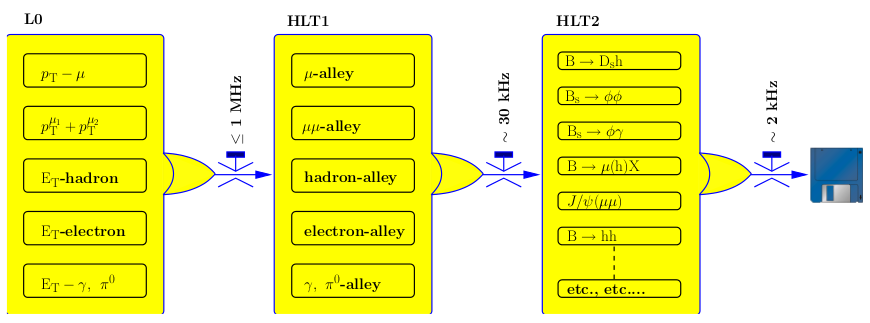
\includegraphics[scale=0.7]{figs/HLT.png}
\caption{Flow-diagram of the different trigger sequences~\cite{Alves:2008zz}.\label{fig:lhcb_HLT}}
\end{center}
\end{figure}

Both HLT1 and HLT2 summaries, containing the information of all tracks and vertexes that triggered events, are stored. This allows the study of the trigger performance, as well as of the trigger source of each event. Furthermore, in order to ensure the traceability of the trigger condiions in the off-line analysis, the combination of trigger algorithms with their selection parameters are pre-loaded in the EFF before a fill in a Trigger Configuration Key (TCK). 

\subsubsection{HLT1} 
\label{sec:HLT1}
The main goal of HLT1 is the so-called L0 confirmation, to reconstruct particle in the VELO and T-stations correspondence to the L0 objects, or for neutral particles to confirm de absence of a charged particle that could be associated to these same objects. Different reconstruction sequences (\textit{alleys}) with different algorithms and selection cuts are applied according to the L0 candidate type. The events can pass by more than one alley, provided that they are selected by multiple triggers. 
\subsubsection{HLT2}
At this stage of the trigger, a set of tracks is selected with very broad cuts on their momentum and impact parameter, and used to form composite particles. These are then used for all selections to avoid duplication in the creation of final states. The selections can be exclusive or inclusive, depending on whether the full final state is reconstructed or not. The inclusive triggers are less dependent on the on-line reconstruction, while the exclusive one produces a smaller rate, thus allowing for a more relaxed set of cuts.  
\label{sec:HLT2}

%% online and simulation? 

%\subsection{Performance} % s2
\subsection{Tracking and Vertexing performance}
\label{sec:TrackingPerformance}
In the track reconstruction software the hits in the VELO, the TT, the IT and the OT detectors are combined to form particle trajectories from the VELO to the calorimeters, with the purpose of finding all tracks in the event wihich leave sufficient detector hits. Depending on the subdetectors used for the reconstruction, offline tracks are classified in the following categories (see \ref{fig:lhcb_Tracks}): 

\begin{itemize}
\item \textbf{Long tracks}: those that traverse the VELO, the TT and the T-stations, hence having the most precise momentum determination. 
\item \textbf{Upstream tracks}: those traversing only the VELO and TT stations. Generally, they have lower momentum and are bent out of the detector acceptance by the magnetic field. Nevertheless, they pass through the RICH1 detector. Hence, they may generate Cherenkov photons, nd cn be used to understand backgrounds. Besides, they can also be used for flavour tagging, albeit their momentum resolution is poor.
\item \textbf{Downstream tracks}: travering only the TT and T stations. The most relevant cases are the decay products of $K_S^0$ and $\Lambda$ that decay outside of the VELO acceptance. 
\item \textbf{VELO tracks}: measured in the VELO only and typically with large angle, or backward trakcs. They are useful for the primary vertex reconstruction. 
\item \textbf{T tracks}: the ones measured in the T stations, typically produced in secondary interactions, but useful for the global pattern recognition in RICH2. 
\end{itemize}
For $K_S^0$ reconstruction, only long tracks and downstream tracks are used. 

\begin{figure} [htb!]
\begin{center}
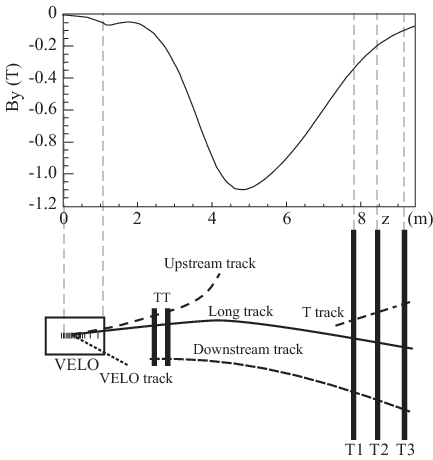
\includegraphics[scale=0.6]{figs/TrackTypes.png}
\caption{Schematic illustration of the various track types. For reference the main \textit{B}-field component ($B_y$) os plotted above as a function of the \textit{z} coordinate~\cite{Aaij:2014jba}.\label{fig:lhcb_Tracks}}
\end{center}
\end{figure}

For the track reconstruction algorithm, track \textit{seeds} are used as starting points. These are the initial track candidates in the VELO and T stations, where the magnetic field is low. Their trajectories are refitted using the Kalman filter~\cite{Fruhwirth:1987fm}, that accounts for multiple scattering and energy loss. The quality os such fitting is monitored using the $\chi^2$ of the fit and the \textit{pull} distribution for the different parameters. 

The pattern recognition performance is evaluated in terms of efficiencies and ghost rates. The efficiencies are the ratio of successfully reconstructed tracks over the total amount of reconstructible tracks. A track is considered recontructible if it has a minimum number of hits in the relevant subdetector, and \textit{successfully reconstructed} if at least 70\% of such hits originate from a single MonteCarlo (simulated) particle. Otherwise, it is considered a \textit{ghost track}. 

Figure \ref{fig:lhcb_TrackEfficiency} shows this efficiency as a function of two kinetic variables, namely the momentum, \textit{p}, and the pseudorapidity, \textit{eta}, for 2011 and 2012. The performance in the 2012 data is slightly worse, which is partially due to the higher hit multiplicity at the higher centre-of-mass energy~\cite{Aaij:2014jba}. The average efficiency is above 96\% for $5 \rm GeV/c < p < 200 \rm GeV/c$, $2 < \eta < 2$, thus covering the LHCb phase space. 

\begin{figure} [htb!]
\begin{center}
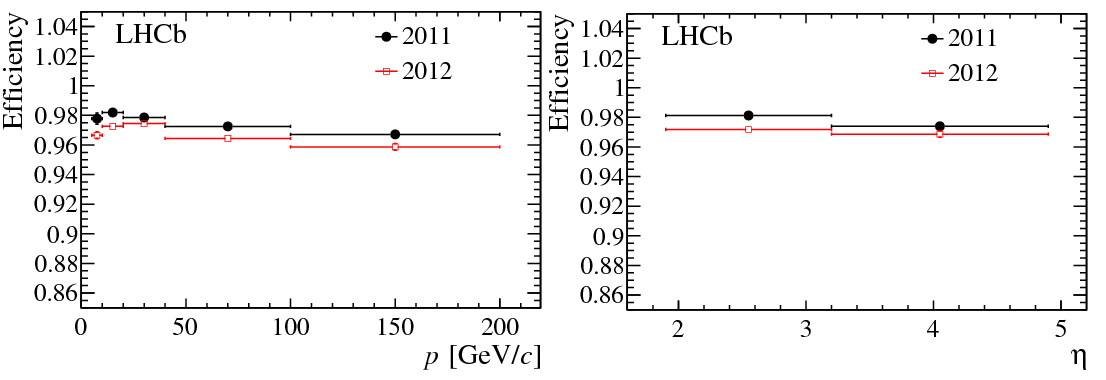
\includegraphics[scale=0.5]{figs/Efficiency_p_eta.png}
\caption{Tracking efficiency on muons from $J/\psi$ as a function of momentum (left) and
pseudorapidity (right). Black points correspond to 2011 data and red 2012 data
~\cite{Aaij:2014jba}.\label{fig:lhcb_TrackEfficiency}}
\end{center}
\end{figure}

As for the relative momentum resolution, as it is shown in \ref{fig:lhcb_Resolution} for two muons coming from a $J/\psi$,it is better (about 5 per mille) for low-momentum than for high-momentum (about 8 per mille) ranges. Hence, the best performances in terms of momentum resolution are achieved for long tracks, as said before. 

\begin{figure} [htb!]
\begin{center}
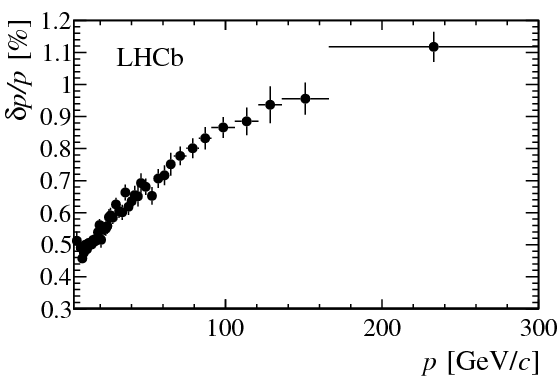
\includegraphics[scale=0.5]{figs/Resolution_p.png}
\caption{Relative momentum resolution versus momentum for long tracks in data obtained using $J/\psi$ decays~\cite{Aaij:2014jba}.\label{fig:lhcb_Resolution}}
\end{center}
\end{figure}

In order to assess the vertexing performance at LHCb, two main quantities are examined: the primary vertex (PV) resolution, and the impact parameter. The PV resolution is measured by comparing two independent measurements of the vertex position in the same event. This is achieved by randomly splitting the set of tracks in an event into two and reconstructing the PVs in both sets. 

The impact parameter (IP) of a track is defined as its distance from the primary vertex
at its point of closest approach to the primary vertex. Particles resulting from the decay
of long lived \textit{B} or \textit{D} mesons tend to have larger IP than those of particles produced at the primary vertex. Selections on IP and the IP $\chi^2$ are extensively used in LHCb analyses to reduce the contamination from prompt backgrounds. Consequently, an optimal IP resolution and a good understanding of the effects contributing to the IP resolution are of prime importance to LHCb performance~\cite{Aaij:2014jba}.

The IP resolution is governed by three main factors: multiple scattering of particles by
the detector material; the resolution on the position of hits in the detector from which
tracks are reconstructed; and the distance of extrapolation of a track between its first hit in the detector and the interaction point. The minimisation of these factors is achieved in the design of the VELO~\cite{Aaij:2014jba}. %The sensors are positioned close to the beams, separated from them by only a thin aluminium foil. The first active strips are only 8 mm away from the beams during physics collisions. 

The left part of figure \ref{fig:lhcb_PV_IP} shows the PV resolution in the \textit{x} and \textit{y} direction as a function of the number of tracks. It can be seen that in both cases it immproves with the number of tracks. The right part shows the IP resolution in the \textit{x} direction as a function of the inverse of the transverse momentum. Very good resolution is achieved in the VELO, thanks to the silicon strips. 

\begin{figure} [htb!]
\begin{center}
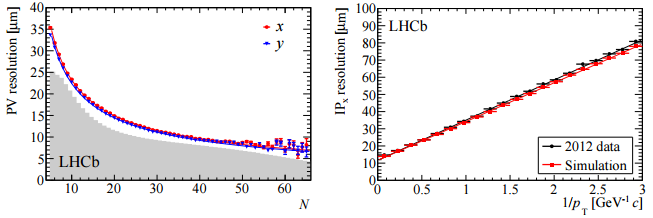
\includegraphics[scale=1.0]{figs/PV_IP.png}
\caption{The primary vertex resolution (left), for events with one reconstructed primary vertex, as a function of track multiplicity. The \textit{x} (red) and \textit{y} (blue) resolutions are separately shown and the superimposed histogram shows the distribution of number of tracks per reconstructed primary vertex for all events that pass the high level trigger. The impact parameter in \textit{x} resolution as a function of $1/p_T$ (right). Both plots are made using data collected in 2012.~\cite{Aaij:2014jba}.\label{fig:lhcb_PV_IP}}
\end{center}
\end{figure}

\subsection{PID performance} %% 2 dias s2
\label{sec:PIDPerformance}
As explained in \ref{subsec:PID}, particle identification at LHCb is performed in 4 different subdetectors. Each one of them gives a different performance that is then further combined into an overall PID performance. 

For the calorimeters the main role is to distinguish photons, electrons and neutral pions. Electrons are differentiated from photons and $\pi^0$ in the fact that they have a track associated before the energetic deposit in the calorimeter, as they are charged particles. Their associated likelihood is estimated using information from the ECAL, the PS and the HCAL. 
In order to separate photons from $\pi^0$, a neural network clasifier is used, trained with samples as pure as possible. Non-converted photons are identified using a photon hypothesis likelihood, employing variables from the different subdetectors (PS and ECAL). %%% DLL?

Both for photons and for electrons, the PID performance is assessed using the log-likelihood difference between the signal hypothesis (photon or electron) versus the background one (hadrons for electrons). In the cae of the electrons, this log-likelihood is computed as the sum of log likelihoods:
\begin{equation}
\Delta \log{\mathcal{L}^{\rm CALO}(e-h)} = \Delta \log{\mathcal{L}^{\rm ECAL}(e-h)} + \Delta \log{\mathcal{L}^{\rm HCAL}(e-h)} + \Delta \log{\mathcal{L}^{\rm PS}(e-h)} 
\end{equation}

This is shown in \ref{fig:PID2}, for different cuts. As expected, the higher momenta particles have higher misidentification rates. 
\begin{figure} [htb!]
\begin{center}
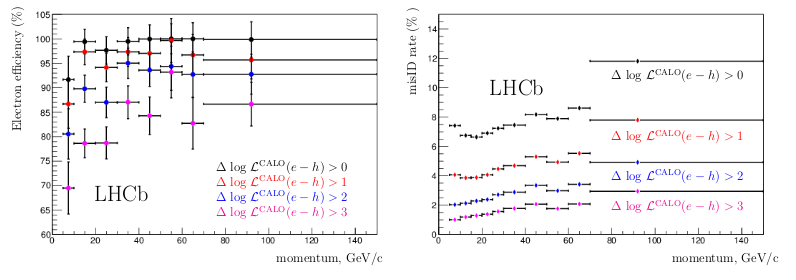
\includegraphics[scale=0.8]{figs/PID2.png}
\caption{Electron identification performances for various $\Delta\log{\mathcal{L}^{\rm CALO}(e-h)}$ cut: electron efficiency (left) and misidentification rate (right) as functions of the track momentum~\cite{Aaij:2014jba}.\label{fig:PID2}}
\end{center}
\end{figure}

%\red{FIGREF} shows the ratio of photon detection efficiencies between converted and non-converted photons coming from the decay of $\pi^0$ mesons for both simuation and data. As it can be seen, simulation properly reproduces the data distribution, and the reconstruction algorithms work equally well in data and simulation., PID1 

As for the RICH, its mission is to distinguish charged hadrons ($\pi$,$K$,$p$). The information thus obtained is used at the final analysis level and as part of the software level of the trigger. Complementary information on charged leptons can also be provided by the RICH. Its performance is evaluated using two variables:
\begin{itemize}
\item The Cherenkov angle resolution, $\theta{(\sigma_C)}$, defined as the resolution of the Cherenkov angle with which the emitted photons can be reconstructed. 
\item The photoelectron yield, defined as the average number of detected photons for each track traversing the Cherenkov radiator media. 
\end{itemize}

Because of te high average track multiplicity in LHCb events, a reconstructed Cherenkov ring will generally overlap with several neighbouring rings. Figure \ref{fig:PID3} shows the Cherenkov angle as a function of particle momentum using information from the raditor for isolated tracks selected in data. As expected, different bands represent different masses, hence different particles. 

\begin{figure} [htb!]
\begin{center}
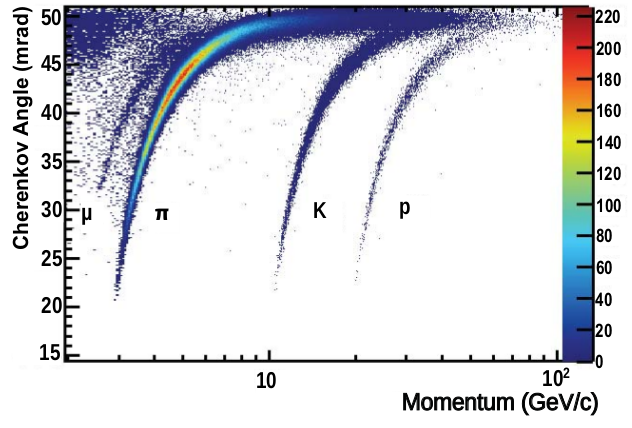
\includegraphics[scale=0.7]{figs/PID3.png}
\caption{Reconstructed Cherenkov angle for \textit{isolated} tracks, as a function of track momentum in the radiator. The Cherenkov bands for muons, pions, kaons and protons are clearly visible~\cite{Aaij:2014jba}.\label{fig:PID3}}
\end{center}
\end{figure}
%%% To determine the RICH particle id performance on data, large samples of genuine pi, K and p tracks are required. 

Figure \ref{fig:PID4} shows the kaon efficiency (kaons identified as kaons) and pion misidentification (pions misidentified as kaons) fraction achieved in LHCb data and simulation, as a function of momentum. The results are shown both optimising efficiency and minimising misidentification rate. 

\begin{figure} [htb!]
\begin{center}
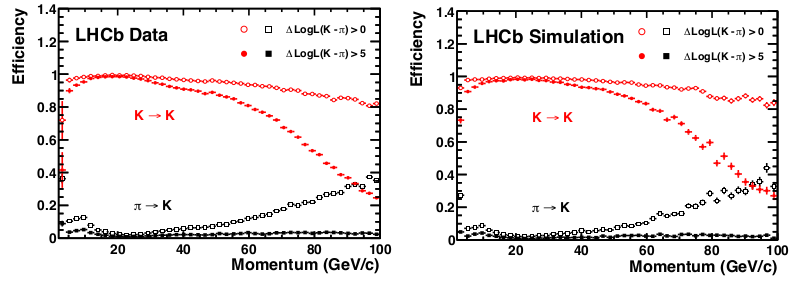
\includegraphics[scale=0.7]{figs/PID4.png}
\caption{Kaon identification efficiency and pion misidentification rate as meaured using data (left) and from simulation (right) as a function of track momentum~\cite{Aaij:2014jba}\red{improve}.\label{fig:PID4}}
\end{center}
\end{figure}

Finally, muons are identified in the muon system. The algorithm is based on the association of hits around its extrapolated trajectory. In this case, the logartihm of the ratio between the muon and non-muon (protons, pions and kaons)  hypothesis, $\Delta\log{\mathcal{L}(\mu)}$ is used as discriminating variable. Figure \ref{fig:PID5} shows, as a function of the track momentum and for different ranges of transverse momentum, the efficiency of the muon candidate selection, and the probabilities of incorrect identification of protons, pions and kaons as muons. 

\begin{figure} [htb!]
\begin{center}
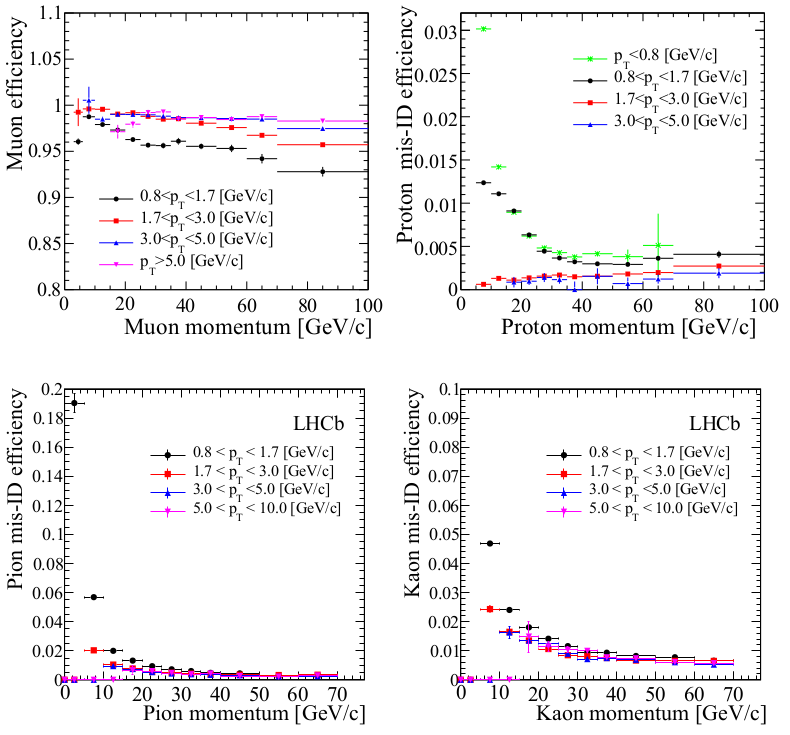
\includegraphics[scale=0.7]{figs/PID5.png}
\caption{Top left: efficiency of the muon candidate selection based on the matching of hits in the muon system to track extrapolation, as a function of momentum for different $p_T$ ranges. Other panels: msiidentification probability of protons (top right), pions (bottom left), and kaons (bottom right) as muon candidate as a function of momentum, for different $p_T$ ranges~\cite{Aaij:2014jba}.\label{fig:PID5}}
\end{center}
\end{figure}

The combined performance of the different PID subdetectors can be either be computed as a sum of the different likelihoods, or using multivariate techniques to get a single probabiity value for each particle hypothesis with different informations corresponding to each sub-system. 


\subsection{Trigger performance} %% 3 dias s2
\label{sec:TriggerPerformance}
As discussed in \ref{sec:Trigger}, the LHCb trigger is composed of two parts, in order to reduce the input rate to an output rate of 2 -5 kHz. The performance of each part is assessed using a data-driven technique with representative samples, to account for inefficiencies due to the simplified reconstruction algorithm, possible misalignments and reduced resolution. 

In the trigger system, an event is considered to be \textit{Trigger on Signal (TOS)} if the trigger objects that are associated with the signal candidate are sufficient to trigger the event. On the contrary, if the event has been triggered by trigger objectos not associated with the signal, it is considered \textit{Trigger Independet of Signal (TIS)}. Notice that events can be both TIS and TOS. The TIS and TOS efficiencies are defined as follows:
\begin{equation}
\epsilon^{\rm TIS(TOS)} = N^{\rm TIS \& TOS}/N^{\rm TOS(TIS)}
\end{equation}

\subsubsection{L0 hardware trigger}
The L0 trigger consists of three independent nits:
\begin{itemize}
\item The L0-Calorimeter trigger, that uses information from the SPD, PS, ECAL and HCAL to compute $E_T$ that particles deposit in clusters of 2x2 cells. From this, a candidate can be \texttt{L0Hadron}, \texttt{L0Photon} or \texttt{L0Electron}. 
\item The L0-Muon trigger, that looks for the two highest $p_T$ muon tracks in each quadrant, with thresholds on the $p_T^{\rm largest}$ and $p_T^{\rm largest} \times p_T^{\rm 2nd largest}$. 
\item The L0-PileUp trigger, used for the computation of the luminosity. 
\end{itemize}

Figure \ref{fig:L0Perf} shows the L0 hadron efficiency for the repreentative channels. As expected, it increases with the transverse momentum. 
\begin{figure} [htb!]
\begin{center}
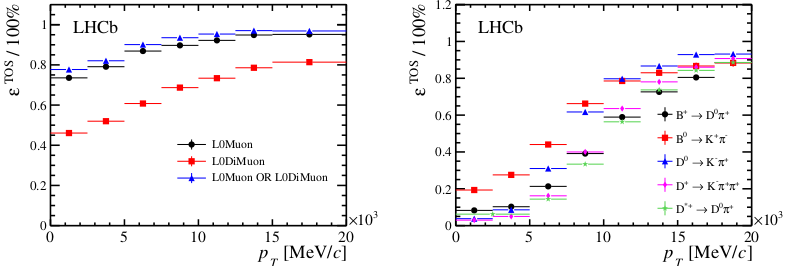
\includegraphics[scale=0.7]{figs/L0Perf.png}
\caption{(left) L0 muon trigger performance: TOS trigger efficiency for selected $B^+ \rightarrow J/\psi K^+$ candidates. (right) L0 hadron trigger performance: TOS trigger efficiency for different beauty and charm decay modes.~\cite{Aaij:2014jba}.\label{fig:L0Perf}}
\end{center}
\end{figure}


\subsubsection{High Level Trigger}
The HLT has a variety of so-called trigger "lines" that consist of selection parameters for specific classes of events. In HLT1, a partial event reconstruction is performed, while in HLT2 the complete event is reconstructed. 

In the first level (HLT1), vertices are reconstructed from a minimum of five intersecting VELO tracks. Vertices within a radius of 300 $\mu \rm m$ of the mean position of the pp-interaction envelope are considered to be primary vertices. During Run 1, the forward track search had a minimum momentum requirement that varied between 3 and 6 GeV/c. Dimuon candidates are either selected based on their mass without any displacement requirement, or based on theiir displacement without the mass restriction~\cite{}. The performance of HLT1 on muonic signatures as a function of $p_T$ of the $B^+$ parent is shown in \ref{fig:HLT1Perf}. 

\begin{figure} [htb!]
\begin{center}
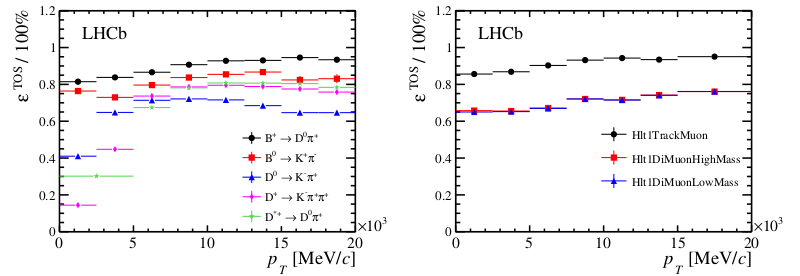
\includegraphics[scale=0.7]{figs/HLT1Perf.png}
\caption{HLT1 inclusive track trigger performance: TOS efficiency for various channels as a function of \textit{B} or \textit{D} $p_T$ (left) . HLT1 muon trigger performance : TOS efficiency for $B^+\rightarrow J/\psi K^+$~\cite{Aaij:2014jba}.\label{fig:HLT1Perf}}
\end{center}
\end{figure}


In the second level (HLT2), long tracks are searched based on VELO seeds, thus simplifying the offline tracking algorithm (because of CPU restrictions). There is a generic beauty trigger, for any partially recontructed \textit{b}-hadron decay, muon triggers, for decays with one or two muons, charm triggers and other exclusive and technical lines. Figure \ref{fig:HLT2Perf} shows the peformance of the $J/\psi$ triggers. %% comments? 

\begin{figure} [htb!]
\begin{center}
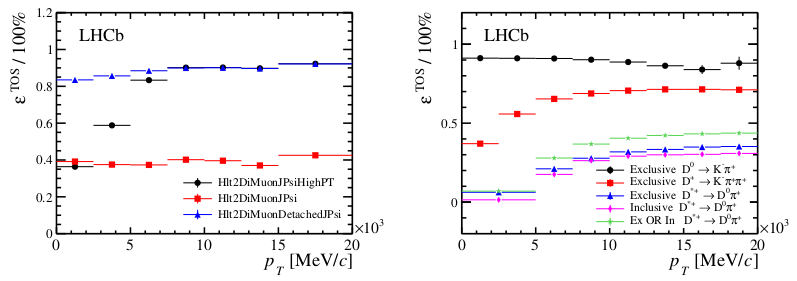
\includegraphics[scale=0.7]{figs/HLT2Perf.png}
\caption{HLT2 muon trigger performance for the $J/\psi$ trigger lines (left). HLT2 charm trigger performance for inclusive and exclusive selections (right).~\cite{Aaij:2014jba}.\label{fig:HLT2Perf}}
\end{center}
\end{figure}

%%\subsection{Experimental conditions} % jueves
%%% data, total luminosity

%%% magnetic field polarity 

\subsection{The LHCb Upgrade} % jueves, viernes, sabado

%%% Motivation: improve sensitivity, detector must be upgraded . fully exploit the potential of the LHC 
%%%update detector with read out at 40 MHz
%%% For this thesis 

The LHCb detector has proven to be an outstanding general-purpose detector in the forward pseudorapidity region. Nevertheless, some of the measurements are still statistically limited. Therefore, in order to fully exploit the potential of LHCb, an increase in the luminosity is required. This leads to the need of upgrading some of the subdetectors, since the upgraded detector is expected to collect 50 $\rm fb^{-1}$ during 5 years of data-taking, with a 40 MHz readout (Phase-I of the Upgrade).

For the sake of this thesis, the changes made during the LHCb Upgrade will greatly benefit the sensitivity to rare strange decays, as the trigger limitation will disappear. Also, a significant improvement in the $\phi_s$ measurement is expected. Prospects for the golden modes on these fields can be seen in \ref{fig:prospects}.

\begin{figure} [htb!]
\begin{center}
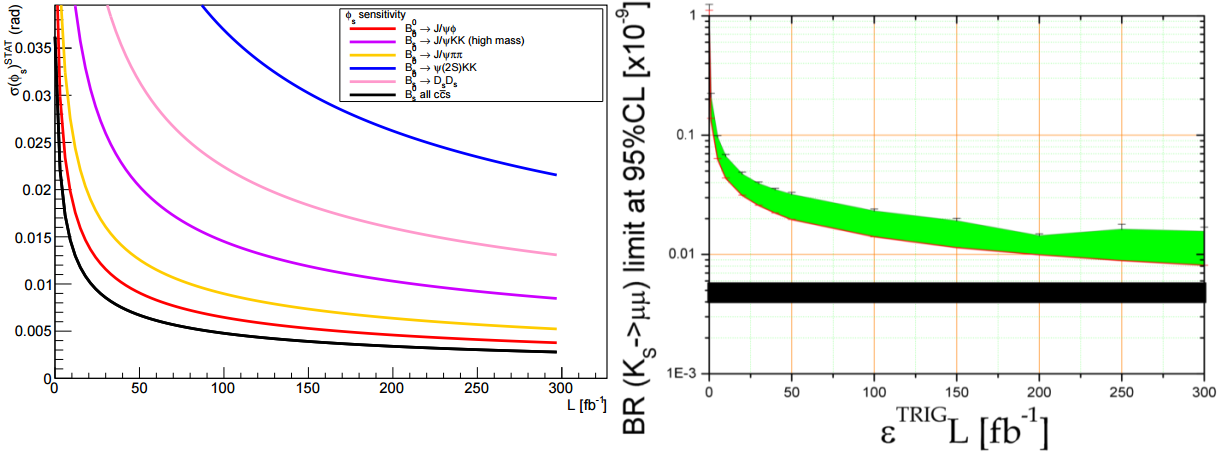
\includegraphics[scale=0.55]{figs/prospects.png}
\caption{Left: expected sensitivity for $\phi_s$ as a function of the luminosity \red{ref}. Right: Expected limit in $\mathcal{B}(K_S^0 \rightarrow \mu^+ \mu^-)$ from LHCb and upgrades, as a function of integrated luminosity times trigger efficiency~\cite{Santos:2018zbz}.\label{fig:prospects}}
\end{center}
\end{figure}

\subsubsection{Trigger Upgrade} 
The main change that the LHCb trigger will undergo is the replacement of the L0 stage by a software one, the so-called \textit{Low Level Trigger} (LLT), modified to run within the new readout architecture. It selects events containing clusters with high transverse energy in the calorimeters or tracks with high transverse momentum in the muon detector. A much larger LLT rate will be alowed, leading to a much larger rate to storage. Hence, the main limits will be processing power and bandwith. The front-end electronics will be upgraded as well to allow reading events at the LHC clock rate. More details can be found in~\cite{LHCbCollaboration:2014vzo}. 
%%\red{hadronic final states? (nota de Lars)}

%% Limits on processing power, bandwith
\subsubsection{VELO Upgrade} %%% jueves
The LHCb upgrade requires the VELO to have an excellent vertex resolution and two track separation, with fast pattern recognition capabilities. Moreover, because of the high luminosity, it has to have a sufficient radiation hardness to guarantee the performance throughout all the data-taking period. Besides, the upgraded trigger discussed before strongly relies on this subdetector. 

In order to cope with these requirements, two alternatives were  proposed:
\begin{itemize} 
\item A fine-pitched silicon strip detector, similar to the current design, with improved cooling and a new ASIC.
\item A hybrid pixel detector, called \textit{VeloPix}, that uses the Timepix chip\red{~\cite{LLOPART2007485}}. 
\end{itemize}
Being the latter the one chosen for the Upgrade. The layout of the upgraded VELO can be seen in \ref{fig:VELOUPGRADE}. 


\begin{figure} [htb!]
\begin{center}
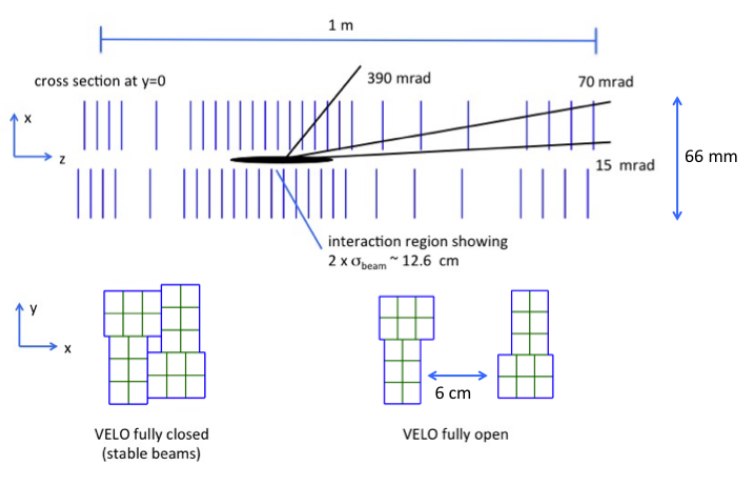
\includegraphics[scale=0.7]{figs/VELO_Upgrade.png}
\caption{Schematic layout of the upgraded VELO.\label{fig:VELOUPGRADE}}
\end{center}
\end{figure}
 
\subsubsection{PID Upgrade}

As discussed before, the PID performance is crucial for the LHCb physics programme. Thus, its upgrade becomes of great importance. 

The overall structure of the RICH will remain unchanged. In RICH1, the aerogel will be removed, as the efficiency gained by its removal outweighs the improvement on the PID provided by it. The HPDs will be replaced by commercial multianode photomultipliers (MaPMTs), with external readout electronics. Alternatively a lens system may be used there, to re-focus the Cherenkov images onto the 1-inch tubes and thus reduce the number of tubes required. A new subdetector, still under development, is being considered in order to recover the low momentum particle identification performance. It consists in a time-of-flight system, Time Of internally Reflected Cherenkov Light, TORCH. 

As for the calorimeter, the electronics will be upgraded according to the new requirements. Also the PMTs gains will be reduced (and compensated by a gain increase in the electronics) to ensure a longer lifetime. Regarding the radiation hardness, studies have found the calorimeter resistent enough, even though some of the elements (such as the cells in the inner region of the ECAL) will need replacing in the long-term scale. Both the SOD and the PS will be removed, as they mainly contribute to the L0 trigger.

Finally, the muon system will have its first station removed, and additional shielding around the beam pipe in front of station M2. Similarly to the calorimeter, the electronics will be modified to comply with the new conditions. 

%An adaptation of the HPD, but with external readout electronics, is under study
%as an alternative photon detector.

\subsubsection{Tracking Upgrade} %% viernes
The TT stations will be replaced by a tracking detector composed of new, high-granularity silicon micro-strip planes with an improved coverage of the LHCb acceptance, the \textit{Upstream Tracker} (UT). Behind the magnet, a \textit{Scintillating Fibre Tracker} (SFT) will be built, which is composed of 2.5m long fibres read out by silicon photomultipliers at the edge of the acceptance, replacing the current OT and IT stations. Both new subdetectors can be seen in \ref{fig:LHCbUPGRADE}.

\begin{figure} [htb!]
\begin{center}
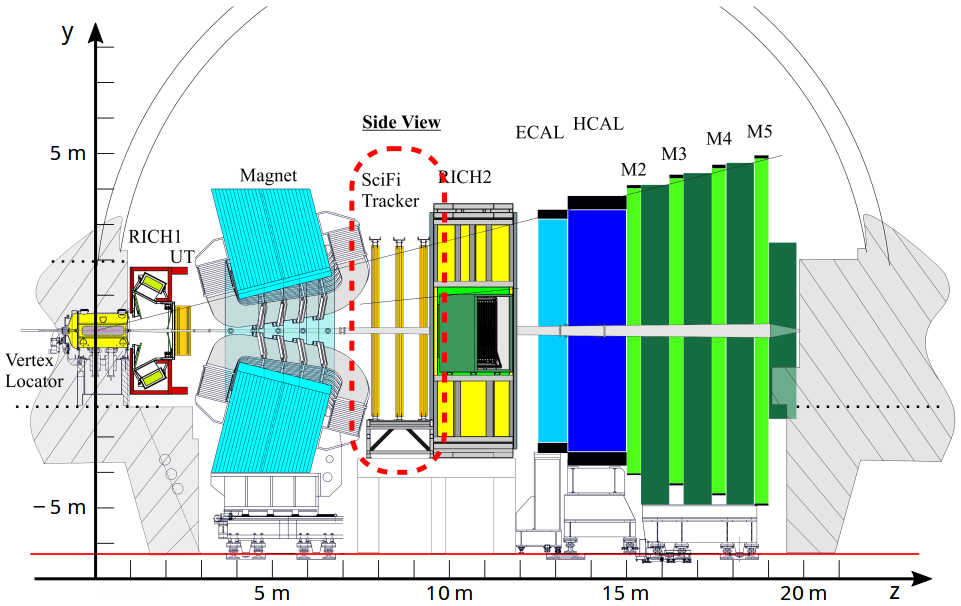
\includegraphics[scale=0.4]{figs/LHCb_upgrade.png}
\caption{Side view of the upgraded LHCb.\label{fig:LHCbUPGRADE}}
\end{center}
\end{figure}

%%% Subdetectors

\subsection{Analysis workflow}
%% rate of several million events per second, Gaudi,introduction to below
Raw data from collisions is taken at LHCb at a rate of several million events per second. A fast, efficient treatment and distribution of such data is thus needed to perform an offline analysis of a given decay channel. For this, C++ tools and algorithms embedded inside the Gaudi~\cite{Mato:691746} project are used. The steps that are followed, together with their correspondance to the different projects inside such framework, are summarised below. 

\begin{enumerate}
\item As explained in \ref{sec:Trigger}, \ref{sec:TriggerPerformance}, a first loose selection is applied to the recorded data with the trigger. The trigger algorithms constitute what is known as the Moore project~\cite{Moore}. 
\item After data is recorded, it is necessary to convert the electronic signals to track and vertices. This was discussed in \ref{sec:Tracking} and \ref{sec:TrackingPerformance}. Particle identification (\ref{sec:PID}, \ref{sec:PIDPerformance}) is also required to properly assign each of these variables to a given type of particle. This whole process is called \textit{reconstruction}, and the group of C ++ LHCb libraries which contain the relevant tools, Brunel~\cite{Brunel}. Proper knowledge alignment of each subdetector is also of great importance at this stage, for which tools under the Alignment project~\cite{Alignment} exist.  %% reconstruction of tracks and vertices, PID (Brunel) alignment of each subdetector 
\item Once all triggered events have been reconstructed, a process is necessary to properly separate them offline according to their physics content. Such process, called \textit{stripping}, consists on a splitting procedure that selects the different decays according to their specific features (final state, PV, mother particle, etc.). Each of the selection criteria are contained in a \textit{stripping line}. The LHCb libraries that take part of this stage are DaVinci~\cite{DaVinci} and Erasmus~\cite{Erasmus}.
\item In order to allow the access to the data, while keeping a backup of it, a distributed system, \textit{Grid}~\cite{Eck:840543} is used by LHCb. Both stripped events and raw data are stored, so as to have the possibility of performing re-stripping and re-reconstruction if needed. Such system is of great computational power, and its spread in computing centers worlwide. 
\item Finally, to properly understand the effects from the detector and the steps before on data, simulation is used. Another important reason for which simulation is crucial is the need of training analysis tool on well-known states.
Simulated Monte Carlo events (MC) are employedfor this, mimicking as much as possible the data. The C++ libraries at LHCb dedicated to the MC production
are contained in Gauss~\cite{Gauss}, which is a collection of libraries for physics simulation based on Gaudi and with specialised algorithms and tools for generators (PYTHIA~\cite{Sjostrand:2006za}, EvtGen~\cite{Ryd:2005zz} ...) and detector simulation (Geant4 ~\cite{Agostinelli2003250}).
The MC events can be further classified as follows:
\begin{itemize}
\item Minimum Bias: keep all events generated by PYTHIA: elastic, diffractive, inelastic.
\item Inclusive: extract events generated by PYTHIA with at least one \textit{b} or \textit{c} hadron in 400 mrad with respect to the LHCb \textit{z} axis. If all of these hadrons have $p_z < 0$, flip the whole event.
\item Signal: extract events generated by PYTHIA containing at least one specific particle in 400 mrad. Again, if the candidate has $p_z < 0$, flip the whole event. In the case of \textit{b} hadrons and to speed up the generation, if the interaction contains the \textit{b}, repeat the hadronisation process of PYTHIA until the interaction contains the correct particle.
\end{itemize}
\end{enumerate}


		
